201. \begin{figure}[ht!]
\center{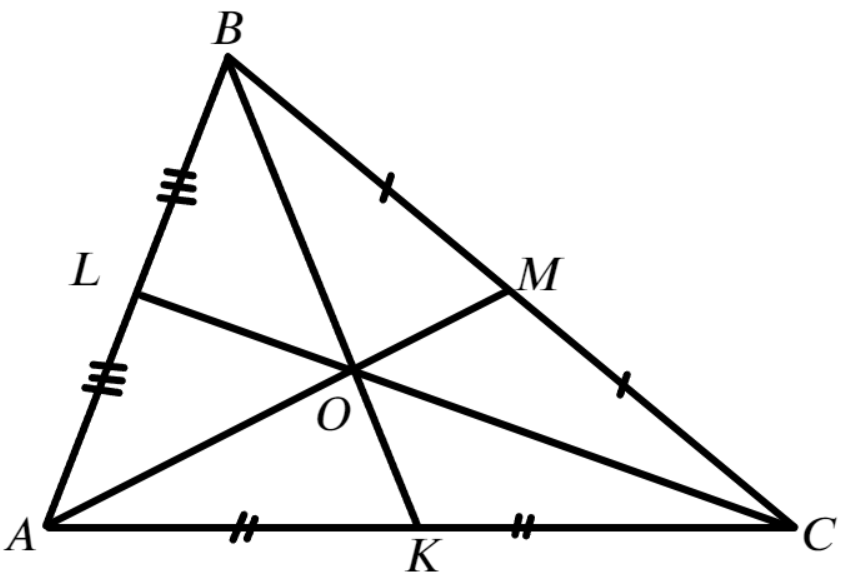
\includegraphics[scale=0.35]{g8-201.png}}
\end{figure}\\
Проведём третью медиану $CL.$ У треугольников с общей высотой и одинаковыми основаниями площади равны, поэтому $S_{\Delta BOM}=S_{\Delta COM}=x,\
S_{\Delta AOK}=S_{\Delta COK}=y,\ S_{\Delta BOL}=S_{\Delta AOL}=z.$ Также $S_{\Delta CBL}=S_{\Delta CAL},$ откуда $2x+z=2y+z,$ поэтому $y=x,$ то есть $S_{\Delta AOK}=S_{\Delta BOM}.$\\
